
\chapter{Related work}

\section{Central pattern generator (CPG)}

Biologists often assume that vertebrate locomotion is controlled by a Central Pattern Generator (CPG) that can automatically generate complex control signals to coordinate muscles during rhythmic movements, such as walking, running, swimming, and flying. CPGs are neural networks capable of producing coordinated rhythmic activity patterns without any rhythmic inputs from sensory feedback or higher control centers. In general, locomotion organized such that CPGs are responsible for converting commands from high-level centers(the motor cortex, cerebellum) to low-level patterns of flexor and extensor movements\cite{ref1}. 

Robotics also tries to solve the problem of locomotion for robots. In the literature, there are two main approaches for the design of locomotion control systems such as kinematic and dynamic mathematical models and biologically inspired approaches\cite{ref1}. The first one tries to calculate joint speed and angel in advance, based on a mathematical model using observation for the environment and robot dynamics \cite{ref10}. The second approach tries to mimic the center of animals' locomotion and create a CPG model that will produce walking patterns. The first approach relies on a complex model and hard to adapt. Since biologists have made major advances in understanding animal locomotion, recent robotics models showed promising results with different legs configurations\cite{ref11}\cite{ref12}

There are several approaches to model CPG. The first one is detailed biophysical models. There are usually based on a system of differential equations that describe how ion pumps and ion channels influence membrane potentials and the generation of action potentials \cite{ref2} \cite{ref3} \cite{ref4}. Hodgkin–Huxley model \cite{ref1_2}(also termed H–H model) developed in the early 1950s is the most popular. However, it is very complicated and computationally expensive for computer simulations involving large populations of neurons. Because of it, most models concentrate on the detailed dynamics of small circuits. The second one uses more abstracted versions of neurons. One of the earliest models of an abstracted neuron is the integrate-and-fire model\cite{ref5}\cite{ref6}. These models focus on how a rhythmic activity is generated by network properties (e.g., half-center networks) and how different oscillatory neural circuits get synchronized via interneuron connections. The disadvantage of this model is that it implements no time-dependent memory present in natural neuron systems. Another approach is to represent CPG as a dynamical system of coupled, nonlinear oscillators. As opposite to neural oscillators, nonlinear oscillators do not have clear biological meanings. According to Junzhi Yu\cite{ref7} typical oscillator models: Matsuoka NO, Cyclic Inhibitory NO, Kuramoto Oscillator, Wilson–Cowan NO, Hopf Oscillator. \cite{ref8} \cite{ref9}

\section{Spiking neural networks}
The human brain has remarkable properties such as analog computation, low power consumption, fast inference, event-driven processing, online learning, and massive parallelism. SNNs model architecture tries to mimic these properties. Because spike events are sparse and have high information content, we could significantly reduce the power consumption of parts of networks that do not receive signals. \cite{ref13}  Similarly, human brains do not use all neurons simultaneously, but only regions needed for current tasks. This same advantage is maintained in hardware \cite{ref14} \cite{ref15}. Thus, it is possible to create low energy hardware based on the property that information is sparse in time and concentrated in spikes. It is one of the biggest advantages of SNNs.

Several models of spiking neurons and SNN have developed so far, e.g.: Hodgkin–Huxley’s model  \cite{ref16}; Spike Response Models\cite{ref17}\cite{ref18}; Izhikevich models \cite{ref19}. However, the vast majority of research on SNNs has been limited to very simple and shallow network architectures on relatively simple digit recognition datasets like MNIST, while only a few works report their performance on more complex standard vision datasets like CIFAR-10. The multi-layer neural architecture in the primate’s brain has inspired researchers to concentrate on the depth of ANNs instead of using shallow networks with many neurons. Theoretical and experimental results show better performance of deep rather than wide structures. This inspired research of deep SNNs. Despite their recent success in image processing tasks using similar CNN architecture, they still cannot beat the corresponding SOTA results of DNN models. One could argue that datasets used for evaluation are more suitable for the DNNs model as they work on frame-level, unlike the SNNs model that require preprocessing frames to spikes data.

Nevertheless, the biggest problem for deep SNNs is the training process. Because spikes signals are sparse and not differentiable, we can not apply backpropagation to train a model. There exist three ways for SNN learning: 1) unsupervised learning such as spike timing-dependent plasticity (STDP); 2) indirect supervised learning such as ANNs-to-SNNs conversion; 3) direct supervised learning such as gradient descent-based backpropagation. However, by far, most of them limited to very shallow structures (network layer less than 4) or toy small datasets (e.g., MNIST, Iris), and little work points to direct training deep SNNs due to their challenges. There is work in progress to develop practical learning algorithms and efficient programming frameworks.\cite{ref20}

Research of CPG models using spiking neural networks(SNNs) mostly focused on the robotics domain to create a locomotion model for different robots. The primary motivation for using SNNs is to reduce the power consumption of embedded devices used to run the robot. Some approaches use Christiansen Grammar Evolution to estimate the spiking neural network's weights and synaptic connections and deploy the FPGA model (Field Programmable Gate Array), which shows excellent performance gains.\cite{ref21} Reinforcement based stochastic weight update could also be used to train on SNNs that runs on a lightweight raspberry pi(\cite{ref22}. The authors' model converges to the desired bio-observed tripod in 70\% of the cases, while in other cases, it converges to suboptimal gaits that can still enable the locomotion. Some of the research focus more on engendering and deployment of SNNs on specific hardware as SpiNNaker boards and do not describe the model learning process \cite{ref23} \cite{ref24}.

\section{Research focus}
Most of the work related to SNNs and CPG are related to robotics and hardware implementation. We are solving the problem of effective locomotion. The motivation of the work is to build neurobiological models of animal CPGs using spiking neural networks. Instead of learning parameters using evolution strategies or reinforcement learning to build an efficient robot, this is a supervised learning task to build close to a biological system. The resulting model should be comparable with real biological CPGs and other low-level models like H-H or integrate-and-fire models. 

\section{Problem Setting and Approach to Solution}
CPGs are self-sufficient networks that could produce output without any sensory input signal. They receive orders from the higher-order system(Corebal cortex, Basal ganglia). The expected speed of locomotion or types of gaits passed to CPG that converts it to produce a muscle phase pattern that achieves the required motion without the supervision of conciseness as shown in Fig.~\ref{fig2}. These patterns are then stable in time till later commands are received. Signals from environmental sensors could alter flexor and extensor phase patterns without intervention from higher-order systems. For example, we could walk without thinking about moving each muscle and avoid minor obstacles reflexively.

\begin{figure}
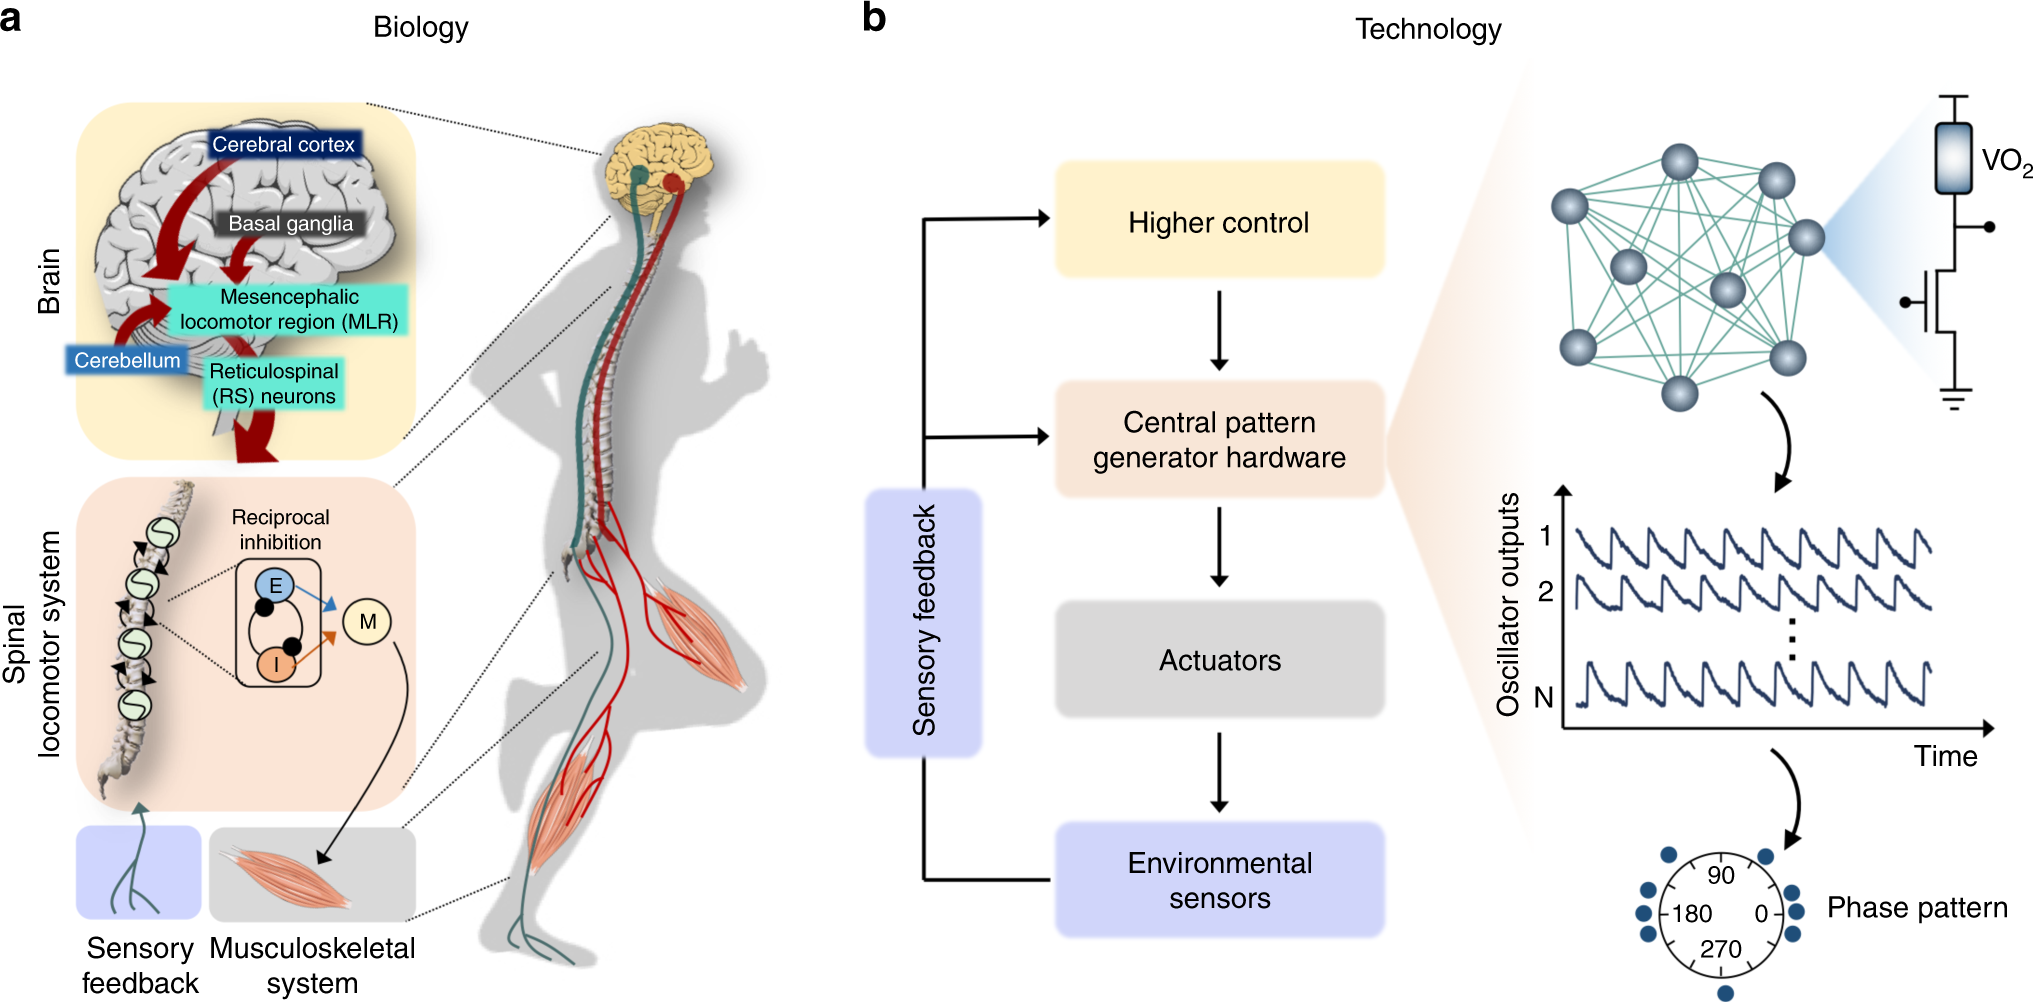
\includegraphics[width=\textwidth]{images/cpg_img.png}

\captionsource{Human locomotion system}{ https://www.nature.com/articles/s41467-019-11198-6/figures/1} \label{fig2}

\end{figure}

The movement of the animal, for example, cat, can be described as a sequence of phases stance and swing for limbs, where the stance is the duration of contact with the surface, and swing is the time in the air. As an animal moves faster, this cycle of phases shortens. Research by Halbertsma \cite{ref24_1} showed that it was mainly achieved by a decrease in stance duration while swing duration stayed mostly unchanged(example Fig.~\ref{fig3} ). Because phase-duration characteristics are integral property of motion initial test for synthetic CPG is to meet the same properties.

\begin{figure}
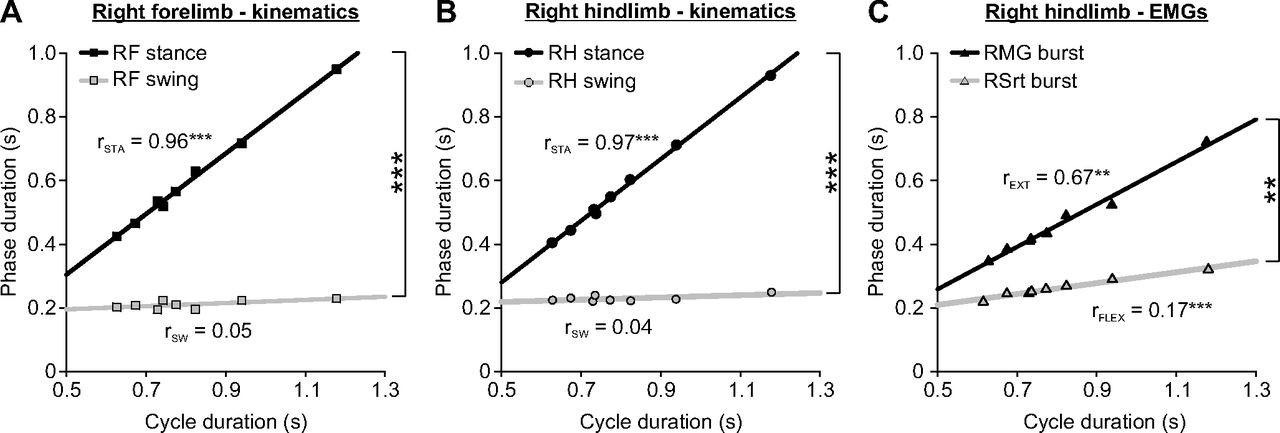
\includegraphics[width=\textwidth]{images/images_large_z9k0091424000003.jpeg}

\captionsource{Phase-duration characteristic}{ https://journals.physiology.org/cms/10.1152/jn.00524.2013/asset/images/large/z9k0091424000003.jpeg} \label{fig3}

\end{figure}


The task is to create a model that receives low dimensional input like the desired speed of an animal and produces a never-ending pattern in the same way that biological CPG does. We will use an average of 1000 steps from 9 different rats for the training and validation, which take up to 100 Gb of memory. The optimization task is to minimize the difference between real rat muscle neuron activation and generated one. Nengo framework will be used to build the CPGs model using SNNs. Spiking models are asynchronous, so input data has a time dimension. There are two ways data could be represented. In the first one, some random synchronized patterns with encoded speed will always feed to the network. Another approach would only give speed change signals once needed and empty signal any other time. There are also different approaches to train SNNs network. The research hypotheses is that SNNs could generalize well to biological CPGs.

\endinput